\section{Iterative Solvers}
\label{sec:iterative_solvers}

The goal of an iterative method is to generate a sequence of increasingly accurate approximate solutions $\hat{x}$ for a linear system $Ax=b$. In such a framework, the matrix $A$ is typically only involved in terms of matrix-vector multiplications, which can be calculated in order of $\mathcal{O}(n^2)$ for a dense matrix \cite{golub_matrix_2013}. Therefore, as long as a desired accuracy can be achieved by a short sequence of approximate solutions, iterative methods are considerably faster than direct solvers (which require $\mathcal{O}(n^3)$). Such techniques are especially common in the context of sparse matrices, where the calculation of the matrix vector product can achieved in (almost) linear complexity.

Many classical iterative methods, such as Jacobi or Gauss-Seidel (see \cite{golub_matrix_2013} or \cite{saad_iterative_2003}) are based on a \textit{splitting} of the original matrix $A$:
\begin{equation}
\label{eqn:splitting}
    A = M - N
\end{equation}

\noindent and thus the iterative solutions can be created by:
\begin{equation}
    Mx^k = Nx^{k-1} +b = (M-A)x^{k-1}+b
\end{equation}

\noindent While this might just look like a regularization of the original problem, the trick to achieving a reduced complexity is in how to choose the splitting in Equation~\hyperref[eqn:splitting]{\ref{eqn:splitting}}. The matrix $M$ has to be chosen in such a way, that its characteristics (for example diagonal structure in Jacobi and lower triangular structure in Gauss-Seidel iterations) allow for an inversion at a lower cost then the original matrix $A$. However, an additional requirement for such methods to be practical is that they must converge (i.e. achieve a desired accuracy) within only a few iterations steps. As remarked in \cite{golub_matrix_2013}, the rate of convergence depends entirely on the eigenvalues of the iteration matrix $G=M^{-1}N$, generally requiring the spectral radios of $G$ to be less than unity:
\begin{equation}
    \rho(G) < 1 \;\;\text{ or }\;\;\ \rho(M^{-1}N)<1
\end{equation}

\noindent Further methods such as the successive over-relaxation (SOR) have been assigned to address this concern by choosing a parameter $\omega$ such that $\rho(M_\omega^{-1}N_\omega)$ is minimized. A good overview of the various methods and their convergence results is provided in \cite{saad_iterative_2003}. 
%TODO
While those classical techniques will be revisited in chapter..., they are rarely used in practice because the error decays too slowly and many iterations are needed before they converge \cite{strang_introduction_2009}.

Instead, most state-of-the-art iterative solvers are based on the idea of projecting a $n$-dimensional problem into a lower-dimensional Krylov subspace \cite{golub_matrix_2013}. For a given matrix $A$ and a vector $y$, the associated Krylov sequence is defined as a set of vectors $\{y, Ay, A^2y, A^3y, \dots\}$ and the corresponding $m$-dimensional Krylov subspace $\mathcal{K}_m$ is the space spanned by the first $m$ vectors \cite{trefethen_numerical_1997}:
\begin{equation}
    \mathcal{K}_m(A,y) = span\{y, Ay, A^2y, \dots, A^{m-1}y\}
\end{equation}

\noindent Viewed from the angle of polynomial approximation, a vector $v$ in the Krylov subspace $\mathcal{K}_m$ can be expressed as a linear combination of powers of $A$ times $y$:
\begin{equation}
\label{eqn:poly1}
    v = c_0y+c_1Ay+c_2A^2y+\dots+c_{m-1}A^{m-1}y
\end{equation}

\noindent In other words $v$ is a polynomial in $A$ times $b$ and by defining $p$ as a polynomial of the form $p(z) = c_0+c_qz+c_2z^2+\dots+c_{m-1}z^{m-1}$, the following, compact description can be achieved:
\begin{equation}
\label{eqn:poly2}
v=p(A)b    
\end{equation}

\noindent A Krylov subspace method for solving a linear system will thus attempt to improve a initial solution $x^0$ based on the residual $r^0 = b-Ax^0$ by updating it with such a vector $v \in \mathcal{K}_m(A, r^0)$, which corresponds to:
\begin{equation}
    A^{-1}b \approx x^m = x^0+p(A)r^0
\end{equation}

\noindent Note that even though all Krylov subspace based techniques provide the same type of polynomial approximation, they differ in the constraints used to build these approximation, giving rise to a number of distinct algorithm (see \cite{saad_iterative_2003} for a comprehensive overview) and only a subset will be discussed in this research.



\subsection{Arnoldi's Method}
\label{sec:arnoldi}
This method, first proposed by Arnoldi \cite{arnoldi_principle_1951} enforces the orthogonality condition $p^m(A)y \perp \mathcal{K}_m$ and is applicable to general non-Hermitian matrices. I was originally proposed for the purpose of reducing a dense matrix into Hessenberg from via a unitary transformation. AT its core, it is an algorithm for building an orthogonal basis of the Krylov subspace $\mathcal{K}_m$. However, it was later discovered that it is also an efficient technique for eigenvalue approximation, and was then extended to the solution of linear systems \cite{saad_iterative_2003}. 

\begin{algorithm}[h]
  \caption{Arnoldi's Method}
  \label{alg:arnoldi}
  \SetAlgoLined
  \KwIn{non-singular matrix $A \in \mathbb{R}^{n \times n}$, arbitrary vector $y \in \mathbb{R}^{n}$}
  \KwOut{\\ Hessenberg matrix $H \in \mathbb{R}^{(m+1) \times m}$ \\
  sequence of orthonormal vectors $q^i\in \mathbb{R}^{n}$ where $i = 1, 2, \dots, m$\\
  \hrulealg}
  $q_1= y\:/\norm{y}_2$ \\
  \For{$i = 1$ \KwTo $m$} {
    $w =A\cdot q^i$ \\
    \For{$j = 1$ \KwTo $i$} {
      $H_{j,i} = w^T\cdot q^j$ \\
      $ w = w - H_{j,i}\cdot q^j$}
    $H_{i-1,i} = \norm{w}_2$ \\
    \If{$H_{i-1,i} = 0$}{\Return}
    $q^{i+1} = w/H_{i+1,i}$
  }
\end{algorithm}

\noindent Following the process outlined in Algorithm~\hyperref[alg:arnoldi]{\ref{alg:arnoldi}}, the successive iterates are related by the following formula:
\begin{equation}
AQ_n=Q_{m+1}\tilde{H_m}
\end{equation}
\noindent where $\tilde{H_m}$ is the $(m+1) \times m$ upper-left section of $H$ (and thus also a Hessenberg matrix) and $Q_m$ is:
\begin{equation}
  Q_m =
  \left[
    \begin{array}{c|c|c}
      & & \\
      q^1 &\dots & q^m \\
      & & \\
    \end{array}
  \right] 
\end{equation}

\noindent This is equivalent to:

\begin{equation}
  \left[
    \begin{array}{ccc}
      &  & \\
      & A & \\
      &  & \\
    \end{array}
  \right] \cdot
  \left[
    \begin{array}{c|c|c}
      & & \\
      q^1 &\dots & q^m \\
      & & \\
    \end{array}
  \right] = 
  \left[
    \begin{array}{c|c|c}
      & & \\
      q^1 &\dots & q^{m+1} \\
      & & \\
    \end{array}
  \right]
  \left[
    \begin{array}{ccc}
      H_{1,1} & \dots & H_{1,m} \\
      H_{2,1} & \dots &  H_{2,m}\\
      & \ddots & \vdots \\
      & & H_{m+1, m}  \\
    \end{array}
  \right] 
\end{equation}

\noindent Therefore, the $m$-th column of this equation can be denoted as:
\begin{equation}
    A \cdot q^m = H_{1,m}\cdot q^1+ \cdots + H_{m,m}\cdot q^m + H_{m+1,m}\cdot q^{m+1}
\end{equation}

\noindent From this, it is evident that the vectors $q^i$ form orthonormal bases of the successive Krylov subspaces generated by $A$ and $y$:
\begin{equation}
    \mathcal{K}_m=\langle y, Ay, \dots , A^{m-1}y\rangle = \langle q^1,q^1, \dots , q^{m}\rangle
\end{equation}

\noindent Since Krylov subspace iterations can be analyzed in terms of matrix polynomials (see Equations~\hyperref[eqn:poly1]{\ref{eqn:poly1}} \& \hyperref[eqn:poly2]{\ref{eqn:poly2}}), the same is true for Arnoldi's method. By defining 
\begin{equation}
    P^n = \{\text{monic polynomials of degree }m\}\text{,}
\end{equation}

\noindent that is all polynomials where the coefficient of the term of degree $m$ is 1 and $p \in P^m$, the vector from Equation~\hyperref[eqn:poly2]{\ref{eqn:poly2}} can be written as $p(A)y=A^my-Q_mz$ for some $z \in \mathbb{R}^m$. Due to the orthogonality condition $p^m(A)y \perp \mathcal{K}_m$, Arnoldi's method has the remarkable property that it finds $z$ such that $\norm{A^my-Q_mz}_2$ is minimal. In other words, it solves the least squares polynomial approximation problem $\norm{p^m(A)y}_2 =$ minimum. The full proof behind this characteristic can be obtained from \cite{trefethen_numerical_1997}, but the general intuition is outlined in Figure~\hyperref[fig:arnoldi]{\ref{fig:arnoldi}}.

\begin{figure}[h]
    \centering
    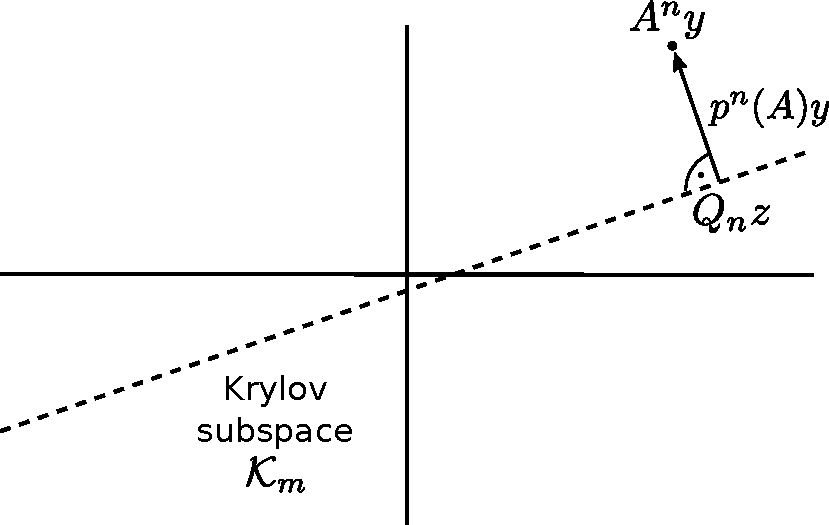
\includegraphics[width=0.6\linewidth]{figures/Arnoldi.pdf}
    \caption{The least squares polynomial approximation problem underlying the Arnoldi iteration as described in \cite{trefethen_numerical_1997}}.
    \label{fig:arnoldi}
\end{figure}

\noindent A final remark on Arnoldi's method has to be made with regards to numerical stability. As can be seen from the pseudo-code given in Algorithm~\hyperref[alg:arnoldi]{\ref{alg:arnoldi}}, the method needs to orthonormalize the resulting vector $w$ against all previous $q^j$'s in each iteration. While several methods are known to achieve this outcome, they differ in terms of speed and numerical stability (for a discussion of the different methods, see \cite{golub} or \cite{trefethen_numerical_1997}). Algorithm~\hyperref[alg:arnoldi]{\ref{alg:arnoldi}} used the Modified-Gram-Schmidt method, but in principle, any other orthonormalization technique can be incorporated into the method. Variants using ordinary Gram-Schmidt or Householder orthogonalization can be obtained from \cite{saad_iterative_2003}.